%%%%%%%%%%%%%%%%%%%%%%%%%%%%%%%%%%%%%%%%%%%%%%%%%%%%%%%%%%%%%%%%%%%%%%%%%%%%%%%%%%%%%%%%%%%%%%%%%%%%%%
%
%   Filename    : chapter_4.tex 
%
%   Description : This file will contain your System.
%                 
%%%%%%%%%%%%%%%%%%%%%%%%%%%%%%%%%%%%%%%%%%%%%%%%%%%%%%%%%%%%%%%%%%%%%%%%%%%%%%%%%%%%%%%%%%%%%%%%%%%%%%
\newcommand{\systemname}{FB Stories } 

\chapter\systemname
\label{sec:\systemname}

This chapter discusses the functional requirements and the overall specifications of the software developed as part of this research, called \systemname. It introduces the software, its objectives, scope and limitations, architecture, and features.

%section~~~~~~~~~~~~~~~~~~~~~~~~~~~~~~~~~~~~~~~~~~~~~~~~~~~~~~~~~~~~~~
\section{Software Overview}
\systemname is a web-based application where Facebook users can generate their own life stories through the data gathered from their Facebook account, with the use of natural language processing (NLP) and generation (NLG) techniques. 

To use \systemname, the user must log in to their Facebook account to access their posts. After a successful login, the user will be asked to approve the permissions set by the software that allows the system to access the user’s personal information as well as the user’s posts which will serve as basis for data extraction. The data extracted will be classified as either direct knowledge or indirect knowledge. Using inferencing techniques, the software will analyze the data that are known to be of direct knowledge, and directly generates a story text out of it later on. For indirect knowledge, text understanding techniques will be applied. All outputs that are generated from this process will be stored in the existing database. 

The software then proceeds to the text generation module, where it determines which elements of the extracted data are appropriate and can be used in generating the life story, and constructs corresponding story text from these data. Once the life story text has been generated, the user will be given the option to save the story into a text file.

The completed life story will contain three parts. The first part contains basic information or facts about the user. These are the data that were either directly extracted from the user’s profile and plotted in the introductory part of the story. The second part contains data extracted from the Facebook posts that were classified and stored into the indirect knowledge base. The second part specifically contains the significant life events based from the posts of the person, while the third part contains the list of preferences of the user inferred from the available list of page likes.

%section~~~~~~~~~~~~~~~~~~~~~~~~~~~~~~~~~~~~~~~~~~~~~~~~~~~~~~~~~~~~~~
\section{Software Objectives}
This section presents the general and specific objectives of \systemname.

\subsection{General Objective}
To generate a story that takes into account the Facebook posts of a user by using natural language processing techniques.

\subsection{Specific Objectives}
\begin{enumerate}
\item To extract needed data from Facebook;
\item To use data processing techniques to analyze the input; 
\item To classify each post according to its type;
\item To use text generation techniques to generate a story;
\item To allow users to save the generated stories into a text file.
\end{enumerate}

%section~~~~~~~~~~~~~~~~~~~~~~~~~~~~~~~~~~~~~~~~~~~~~~~~~~~~~~~~~~~~~~
\section{Scope and Limitations of the Software}

\subsection{Data Extraction}
In retrieving data from a user’s Facebook account, asking for user’s permission is necessary. A successful login to the user’s Facebook account means that the user permits the system to make use of their data. These permissions will be readily set out for the user to approved, and once set, selected options cannot be altered. If the user does not allow the software to access his/her profile with the given permissions, only those public information and public posts of the user will be extracted. 

Only permissions required to gather the user’s personal profile information such as the name, gender and birthday, as well as the details of the posts that the user has posted previously will be needed. \systemname will not extract data from Messenger, as well as information about the people who liked and commented on the user’s posts.

\subsection{Data Processing}
Data processing techniques will only be applicable to Facebook posts which will be further processed to extract relevant data that will be used later during text generation. Personal information such as the name, birthday, location, and what to be known as direct knowledge data, will not be processed by the data processing module and will just be used as is. The data processing module will not perform any verification on the correctness of the user’s personal information. Also, once the input text has been forwarded by the data extraction module to the data processing module, it can no longer be edited or removed.

Posts with hashtags or the text that starts with the `\#' symbol (e.g. \#SampleHashtag) will be removed and will not be processed by the Google Cloud Natural Language API.

For posts with mixed languages, abbreviations and incomplete sentences, the interpretation of these will be limited by what the API can offer \figref{fig:MixedLanguage}. The syntax analysis returned by the Google API will not be checked for the correctness of its output. In this example, ``kain'' is a Filipino word which means ``eat'', thus it should be a verb not a noun. 

\begin{figure}[!htb]                %-- use [t] to place figure at top, [b] to place at the bottom, [h] for here
   \centering                    %-- use this to center the figure
   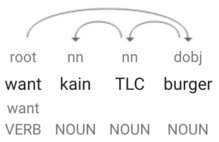
\includegraphics [width=2.5in,height=2.5in,keepaspectratio] {MixedLanguage.png}      %-- include image file named as "disneychart.png" 
   \caption{Sample Incomplete Text with Mixed Languages and Abbreviation.}
    \label{fig:MixedLanguage}
\end{figure}

\subsection{Post Classification}
Much of the data extracted from Facebook cannot be used directly in generating story text, since users tend to post snippets of incomplete, context-based data to show glimpses of their lives. Other posts have no explicit verbs used to describe the event. Thus, the posts must be individually processed to extract the necessary information comprising an event.

Although Facebook has a feature called \textit{Predefined Activities} to enable users to easily  classify their individual posts according to the content, there are currently no tools that can support the extraction of relevant elements from posts that uses this feature. Thus, a post classification algorithm will be needed to classify each Facebook post as either \textit{Celebrating} post, \textit{Travelling} post, \textit{Drinking} post, \textit{Eating} post or \textit{No Event} post. Only the four types of posts are chosen to be used in this research since majority of Facebook posts gathered and analyzed fall under them. Other types of post such as \textit{Reading}, \textit{Listening}, \textit{Watching}, among others may be present in the extracted Facebook posts, but will be ignored and will be tagged as \textit{No Event} posts for this research.

\subsection{Text Generation}
Text generation has three components. One component is responsible for generating the introductory part of the story text, the second component is responsible for generating the body and the last component is responsible for generating the conclusion.

The introduction would contain basic information which will be directly extracted from the user’s profile without going through further processing. All of this information is assumed to be accurate. The body part of the life story will contain events: information which underwent processing and post classification. The conclusion part of the life story will then contain the likes and list of preferences of the user. This will also not undergo data processing module as all information will be used as is.

\subsection{Save to Text File}
The user might want to cherish and read previously generated life stories in the future. This is why it is important to be able to save these generated stories. Text files will only be generated based on the user's instructions. 

The functionality to save to more complex file types such as .docx, or file types that require the use of formatting (e.g. code), will not be included in the software. After successfully saving the generated story into a text file, the user will be solely responsible for the safekeeping and/or dissemination of the file.

For purposes of validating the output of FB Stories and for future research, a copy of the generated life story will also be stored as part of the output of this research. The user will be properly informed of such a practice and their consent will be required through the Informed Consent Form (see Appendix  \ref{sec:appendixh}). In such cases, anonymizing the data, specifically by removing names of people from the generated life story and replacing them with placeholders, is provided as an option for confidentiality.

\clearpage
%section~~~~~~~~~~~~~~~~~~~~~~~~~~~~~~~~~~~~~~~~~~~~~~~~~~~~~~~~~~~~~~
\section{Architectural Design}
\figref{fig:AD} shows the architectural design of the \systemname.

\begin{figure}[!htb]                %-- use [t] to place figure at top, [b] to place at the bottom, [h] for here
   \centering                    %-- use this to center the figure
   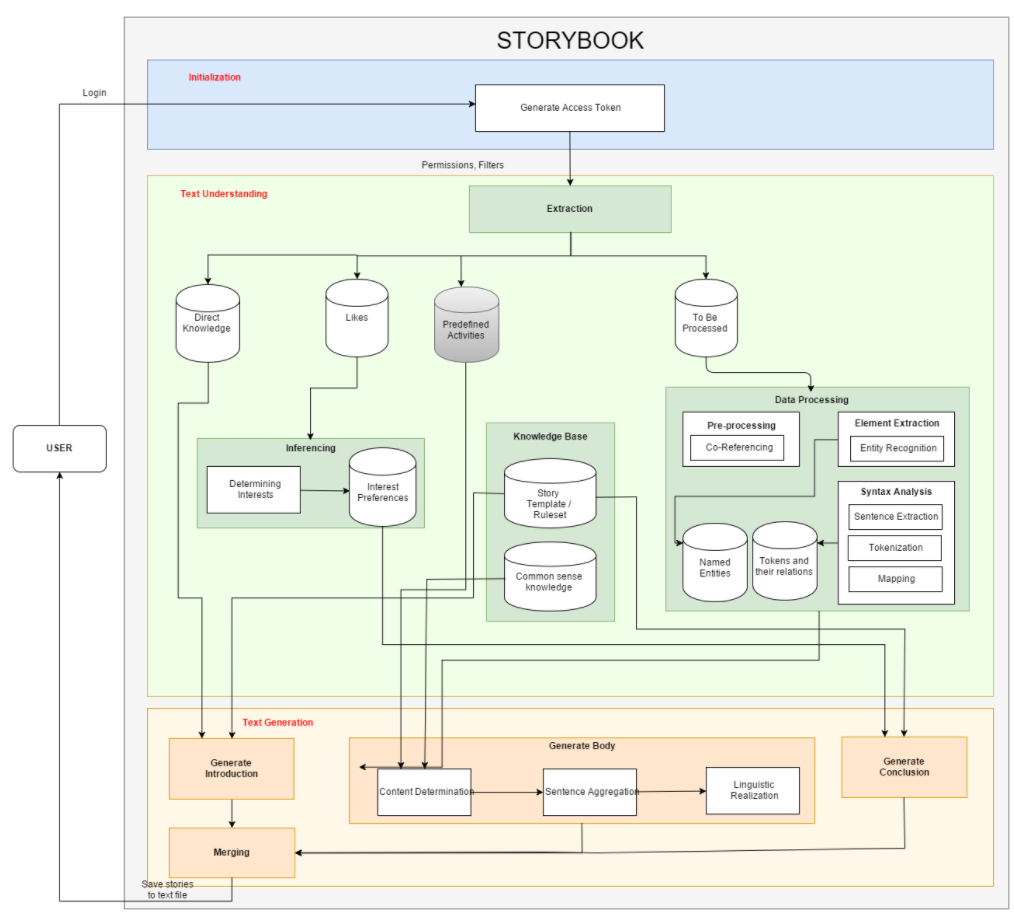
\includegraphics [width=\textwidth] {AD.png}      %-- include image file named as "disneychart.png" 
   \caption{System Architecture of \systemname}
    \label{fig:AD}
\end{figure}

\subsection{User}
\textit{Part of: Startup} \newline \newline
The user, via the use of the Facebook Login API \cite{FacebookLogin}, gives his/her login credentials to allow their Facebook data to be extracted for use in this application and research, and logs into the application. 

Over the course of the software flow, the user can, at any time, choose to stop the extraction or the use of their data, effectively canceling any and all active processes.

\subsection{Initialization}
\textit{Part of: Startup} \newline \newline
During initialization, data will be gathered from a user’s Facebook posts. Consent is paramount in this research as the user will have a good amount of their Facebook data extracted in order to be able to create a life story. Therefore the first step is to ensure that the user confirms the permissions they will allow \systemname to use. Facebook allows over thirty (30) individual permissions to be reviewed by the user if an application requires the use of those particular permissions, such as the user’s friends list, About Me section, list of likes, and events, among others \cite{FacebookLogin}. 

After the user goes through each of the permissions and accepts it, Facebook generates an access token, which will be used by Graph API to determine which data can be extracted from the Facebook account of the user.

\subsection{Data Extraction}
\textit{Part of: Text Understanding} \newline \newline
Three types of data need to be extracted and partitioned into: [1] personal info that can be used as is, such as the user’s birthday, town, and list of family members; [2] data which have to be processed such as text posts; and [3] the user’s list of preferences or likes. 

The partitioned data will be stored in seven separate tables: direct\_knowledge, educational\_bg, work, family, to\_be\_processed, likes and events, as shown in \figref{fig:ExtractedDataDB}. 

\begin{figure}[!htb]                %-- use [t] to place figure at top, [b] to place at the bottom, [h] for here
   \centering                    %-- use this to center the figure
   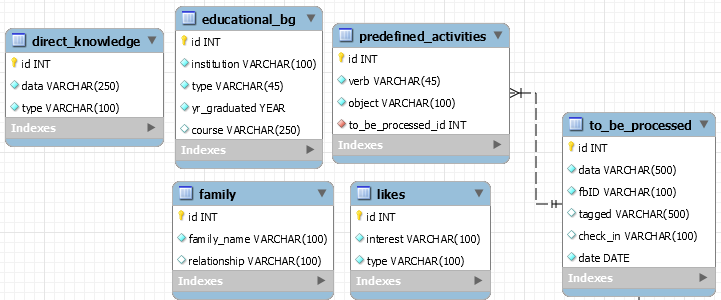
\includegraphics [width=\textwidth] {ExtractedDataDB2.png}      %-- include image file named as "disneychart.png" 
   \caption{Database Design for Storing Extracted Data.}
    \label{fig:ExtractedDataDB}
\end{figure}

Direct knowledge can be extracted from Facebook's About Me section, which contains the personal information of the user. The extracted data also known as the direct knowledge or facts about the user are stored in the \textit{Direct Knowledge Table} (Table \ref{tab:DirectKnowledge}), which contains the following fields:
\begin{itemize}
\item id - unique value that identifies each fact
\item data - the direct knowledge data extracted from his/her Facebook account
\item type - the type of knowledge that describes the data
\item fbID - unique id generated by Facebook for each institution
\end{itemize}
See Appendix \ref{sec:appendixi} for the complete list of types available and a description of each.

Given the sample \textit{About Me} section of a user in Facebook (\figref{fig:AboutMe}), the direct knowledge data that are extracted and stored are shown in Table \ref{tab:DirectKnowledge}:

\clearpage
\begin{figure}[!htb]                %-- use [t] to place figure at top, [b] to place at the bottom, [h] for here
   \centering                    %-- use this to center the figure
   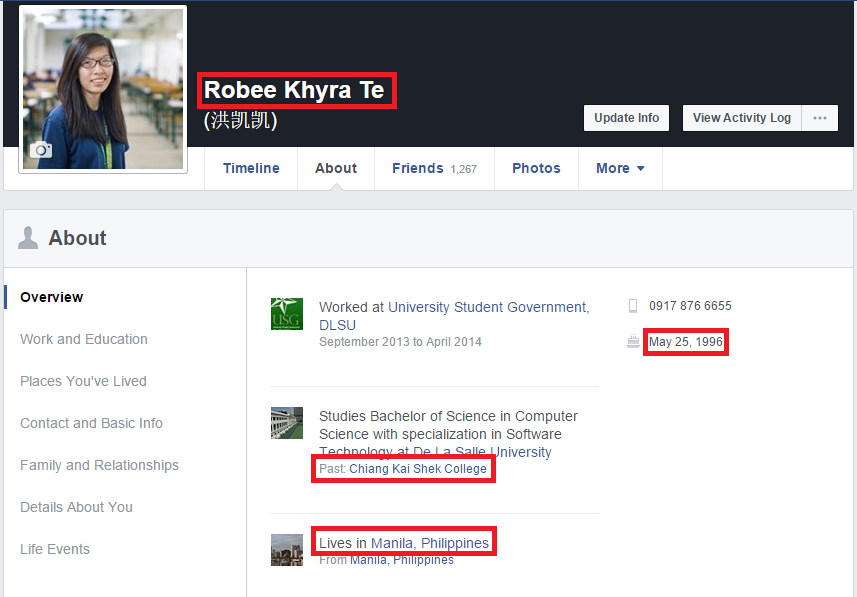
\includegraphics [width=6in,height=4in,keepaspectratio] {AboutMe.png}      %-- include image file named as "disneychart.png" 
   \caption{Sample About Me Section in Facebook}
    \label{fig:AboutMe}
\end{figure}

\begin{table}[ph!]   %t means place on top, replace with b if you want to place at the bottom
\centering
\caption{Sample data in the direct\_knowledge table.} \vspace{0.25em}
\begin{tabular}{|p{1.5cm}|p{2in}|p{1.5in}|} \hline
\textbf{id} & \textbf{data} & \textbf{type} \\ \hline
1 & Robee Khyra Te & name \\ \hline
2 & 1996-05-25 & birth\_date \\ \hline
3 & Manila, Philippines & location \\ \hline
4 & Manila, Philippines & hometown \\ \hline
\end{tabular}
\label{tab:DirectKnowledge}
\end{table}

Educational Background of the user can also be extracted from Facebook's About Me section. These are then stored in the \textit{Educational Background Table} (Table \ref{tab:EducationalBG}), which contains the following fields:
\begin{itemize}
\item id - unique value that identifies each educational level
\item institution - the name of the institution
\item type - the type of educational level
\item year\_started - year enrolled into the institution
\item year\_graduated - year graduated or ended in the institution
\item course - course taken in the said institution
\end{itemize}
See Appendix \ref{sec:appendixi} for the complete list of available types.

\begin{table}[ph!]   %t means place on top, replace with b if you want to place at the bottom
\centering
\caption{Sample data in the educational background table.} \vspace{0.25em}
\begin{tabular}{|p{.5cm}|p{1in}|p{1.5cm}|p{2cm}|p{2.5cm}|p{2cm}|} \hline
\textbf{id} & \textbf{institution} & \textbf{type} & \textbf{year\_ \newline graduated} & \textbf{course} & \textbf{fbID} \\ \hline
1 & De La Salle University & College & null & Bachelor of Science in Computer Science with specialization in Software Technology & 1127420994 \\ \hline
2 & Chiang Kai Shek College & High School & 2013 & null & 4322911189\\ \hline
\end{tabular}
\label{tab:EducationalBG}
\end{table}

Current or previous work of the user can also be extracted from Facebook’s About Me section. These are then stored in the Work Table (Table \ref{tab:work}), which contains the following fields:
\begin{itemize}
\item id - unique value that identifies each work
\item institution - the name of the institution
\item date\_started - year started working in the institution
\item date\_ended - year ended working in the institution
\item location - location of the said institution
\item fbID - unique id generated by Facebook for each work institution
\end{itemize}

\begin{table}[ph!]  
\centering
\caption{Sample data in the work table.} \vspace{0.25em}
\begin{tabular}{|p{.5cm}|p{1.5in}|p{2cm}|p{2cm}|p{2cm}|p{2.5cm}|} \hline
\textbf{id} & \textbf{institution} & \textbf{date\_ \newline started} & \textbf{date\_\newline ended} & \textbf{location} & \textbf{fbID} \\ \hline
1 & University Student Government, DLSU & 2013-09-01 & 2014-04-30 & Manila, Philippines &  
3459628907221
\\ \hline
\end{tabular}
\label{tab:work}
\end{table}


Family members of the user can also be extracted from Facebook's About Me section. These are then stored in the \textit{Family Table} (Table \ref{tab:Family}), which contains the following fields:
\begin{itemize}
\item id - unique value that identifies each family member
\item family\_name - name of the family member
\item relationship - relationship with the user
\end{itemize}
See Appendix \ref{sec:appendixi} for the complete list of available relationships.

\begin{table}[ph!]   %t means place on top, replace with b if you want to place at the bottom
\centering
\caption{Sample data in the family table.} \vspace{0.25em}
\begin{tabular}{|p{1.5cm}|p{2in}|p{1.5in}|} \hline
\textbf{id} & \textbf{data} & \textbf{type} \\ \hline
1 & Jennilyn Wang & sister \\ \hline
2 & Renee Te & sister \\ \hline
\end{tabular}
\label{tab:Family}
\end{table}

Data taken from the user's posts, on the other hand, will require further processing. Graph API will be used to extract data from the user's Facebook posts.

The assumptions for these posts are:
\begin{enumerate} [label=\alph*.]
\item They all contain a description or caption that will be extracted during data processing and may then be used to generate the body part of the story; 
\item The created time of the original post (in case there were no edits made) is assumed to be the time the event happened;
\item If there were edits made, the edited time would be used and considered to determine the time sequence of the posts;
\item The people tagged are used to know that those people are with the user at the time of the event; and
\item All content provided are correct.

\end{enumerate}

\clearpage
\begin{figure}[!htb]                %-- use [t] to place figure at top, [b] to place at the bottom, [h] for here
   \centering                    %-- use this to center the figure
   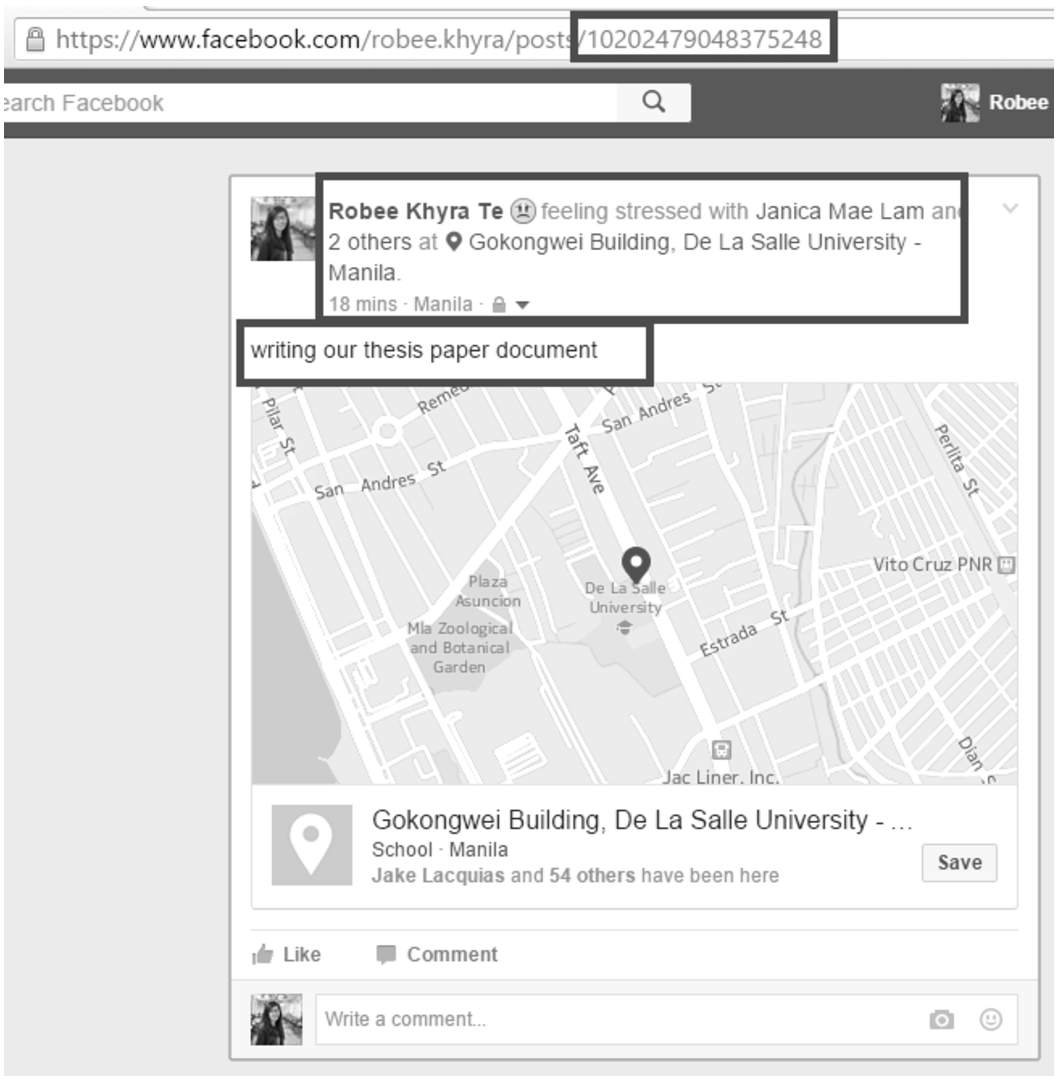
\includegraphics [width=5in,height=4in,keepaspectratio] {SamplePost.png}      %-- include image file named as "disneychart.png" 
   \caption{Sample Post in Facebook}
    \label{fig:SamplePost}
\end{figure}

The \textit{To Be Processed Table} (Table \ref{tab:ToBeProcessed}) will be used to store the description or caption in the user's status and posts, including other relevant information regarding the posts. The following are the attributes of the \textit{To Be Processed} table:
\begin{itemize}
\item id - unique value that identifies each post
\item data - the description/caption extracted from his/her Facebook account
\item fbID - unique id generated by Facebook for each post
\item tagged - comma-separated values representing the friends the user is with for each post
\item place - the place where the event happened
\item city - the city where the event happened
\item country - the country where the event happened
\item year - the year when the post was created
\item month - the month when the post was created
\item day - the day when the post was created
\end{itemize}

\begin{table}[ph!]   %t means place on top, replace with b if you want to place at the bottom
\centering
\caption{Sample data in the to\_be\_processed table.} \vspace{0.25em}
\begin{tabular}{|p{1cm}|p{1in}|p{1in}|p{1in}|p{2cm}|p{1.5cm}|} \hline
\textbf{id} & \textbf{data} & \textbf{fbID} & \textbf{tagged} & \textbf{check\_in} & \textbf{date} \\ \hline
1 & writing our thesis paper document & 102024790 \newline 48375248 & Janica Mae Lam, Camille Saavedra, Alds Hade & Gokongwei Building, De La Salle University - Manila & 2016-11-22 \\ \hline
\end{tabular}
\label{tab:ToBeProcessed}
\end{table}

Given the sample list of user's liked pages section in Facebook (\figref{fig:LikedPage}), the liked data that are stored in the database is shown in Table \ref{tab:Likes}.

\begin{figure}[!htb]                %-- use [t] to place figure at top, [b] to place at the bottom, [h] for here
   \centering                    %-- use this to center the figure
   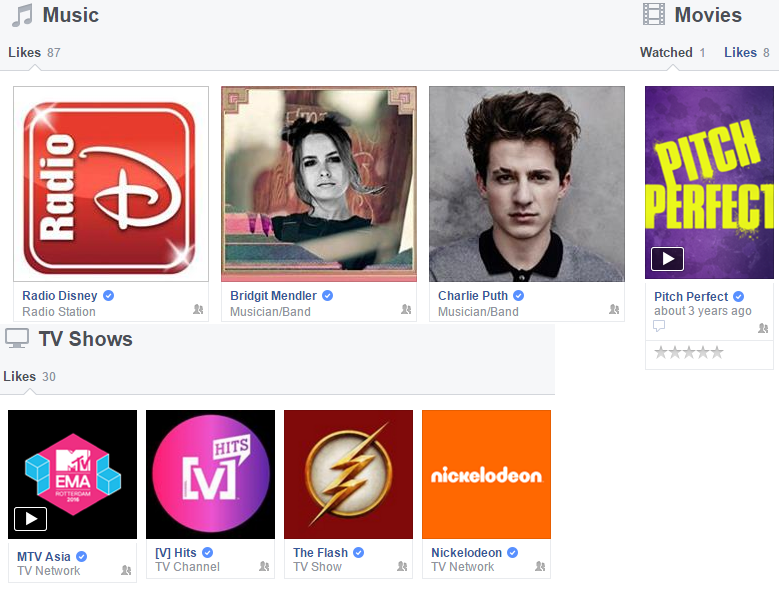
\includegraphics [width=5in,height=4in,keepaspectratio] {LikedPage.png}      %-- include image file named as "disneychart.png" 
   \caption{Sample Interest Preference in Facebook}
    \label{fig:LikedPage}
\end{figure}

The \textit{Likes Table} (Table \ref{tab:Likes}) contains the interest preferences of a particular user in Facebook. This also specifies what time of interest it is.
\begin{itemize}
\item id - unique value that identifies each interest
\item interest - the specific interest liked by the user in his/her Facebook account
\item type - the type of interest that describes the interest
\item fbID - unique id generated by Facebook for ech page
\end{itemize}
See Appendix \ref{sec:appendixi} for the complete list of available types.

\begin{table}[ph!]   %t means place on top, replace with b if you want to place at the bottom
\centering
\caption{Sample data in the likes table.} \vspace{0.25em}
\begin{tabular}{|p{1.5cm}|p{2in}|p{1.5in}|} \hline
\textbf{id} & \textbf{data} & \textbf{type} \\ \hline
1 & Radio Disney & 121 (Radio Station) \\ \hline
2 & Bridgit Mendler & 93 (Musician/Band) \\ \hline
3 & Charlie Puth & 93 (Musician/Band) \\ \hline
4 & Pitch Perfect & 91 (Movie) \\ \hline
5 & MTV Asia & 147 (TV Network) \\ \hline
6 & [V] Hits & 146 (TV Channel) \\ \hline
7 & The Flash & 149 (TV Show) \\ \hline
8 & Nickelodeon & 147 (TV Network) \\ \hline
\end{tabular}
\label{tab:Likes}
\end{table}

Given the sample list of user’s going and interested events in Facebook \figref{fig:events}, the events data that are stored in the database is shown in Table \ref{tab:events1}.

The Events table (Table \ref{tab:events1}) contains all the going and interested events of a particular user in Facebook. It contains the following fields:
\begin{itemize}
	\item id - unique value that identifies each interest
	\item name - the specific interest liked by the user in his/her Facebook account
	\item rsvp\_status - the type of interest that describes the interest 
	\item place - the place where the event took place
	\item city- the city where the event took place
	\item country - the country where the event took place
	\item fbID - unique id generated by Facebook for each event
\end{itemize}
See Appendix I for the complete list of types available.
\clearpage
\begin{figure}[!htb]                %-- use [t] to place figure at top, [b] to place at the bottom, [h] for here
   \centering                    %-- use this to center the figure
   
\includegraphics [width=5in,height=4in,keepaspectratio] {events.png}      %-- include image file named as "disneychart.png" 
   \caption{Sample Events in Facebook}
    \label{fig:events}
\end{figure}

\begin{table}[ph!]   %t means place on top, replace with b if you want to place at the bottom
\centering
\caption{Sample data in the events table.} \vspace{0.25em}
\begin{tabular}{|p{1.5cm}|p{3in}|p{1in}|} \hline
\textbf{id} & \textbf{name} & \textbf{rsvp\_status} \\ \hline
1 & LSCS No Temp Camp &  attending \\ \hline
2 & EmpowHER & attending \\ \hline
\end{tabular}
\label{tab:events1}
\end{table}

\begin{table}[ph!]
\centering
\begin{tabular}{|p{2in}|p{1in}|p{1in}|p{1in}|} \hline
\textbf{place} & \textbf{city} & \textbf{country} & \textbf{FB ID} \\ \hline
STC Campus& Laguna& Philippines& 2343899820\\ \hline
Natividad Fajardo Auditorium, De La Salle University & Manila& Philippines& 2756789237 \\ \hline
\end{tabular}
\end{table}

\clearpage
\subsection{Inferencing}
\textit{Part of: Text Understanding} \newline \newline
Much of the data extracted that suffices as direct knowledge can be directly written to text, such as in the following example: ``Alyana Olivar was born on March 21, 1997.'' This is easily handled during Text Generation. However, some user interests have to be inferred, to answer questions such as, ``how does one determine if one likes music?'' This particular question can be answered by looking at the list of a person's liked pages.

Facebook has six (6) general categories for Pages, and around 100 specific categories. For this study, the top five or six categories with the most pages liked by the user will be written down in the story. This is a combination of both the general and specific categories, since there exists specific categories like ``Band'' and ``Musician/Band'', for example. Narrowing down the categories to the top five allows the life story to focus on the things that the user likes the most.

For instance, if the user named Robee Te likes 87 pages of the category ``Musician/Band'' and it falls under the top five categories of pages she has liked, it can be inferred that she likes music. The top five categories will be later on used in the generation of conclusion. Five sample pages under each category will also be used in the generation of conclusion to provide a better understanding of the user.

\subsection{Data Processing}
\textit{Part of: Text Understanding} \newline \newline
For those data from which knowledge cannot be easily inferred, a more specific procedure of text understanding algorithms is applied. Data processing processes the input and stores them in an abstract representation for use by other modules of \systemname.

The Data Processing comprises the different information extraction tasks explained in detail in Section 3.4, Text Understanding. First, hashtags will be removed as these will not be needed in the story. Only the actual post itself will be used in generating the life events of the user.

After the text has been preprocessed accordingly, different event details such as the noun phrase and verb phrase can now be identified. For every post extracted from Facebook, there can be a presence of several sentences. Stanford CoreNLP will first split the posts to individual sentences. Then, Stanford CoreNLP will perform syntax analysis to each sentence.

The direct objects, the lemmatized verb, as well as other information that were extracted directly from Facebook earlier such as the date of the post, location of the event, and people whom the user is with at the time of the post are then stored in the \textit{Verb Object Table} (shown in Table \ref{tab:sampleVO}) to be used later for the generation of body.

The \textit{Verb Object} table (Table \ref{tab:sampleVO}) contains all the event details in a particular post. It contains the following fields:
\begin{itemize}
	\item id - unique value that identifies each interest
	\item post\_id - value (corresponding to the id from the to\_be\_processed table) representing the post where the sentence is taken from 
	\item verb - the identified verb of the post
	\item noun - the identified object of the post
	\item sentence - an individual sentence from the original post
	\item post\_type - value (corresponding to the id from the post\_type table) representing the post type of the sentence
	\item tagged - the people tagged in the post acquired from the to\_be\_processed table
	\item location - the location where the event took place acquired from the to\_be\_processed table
	\item date - the date when the event happened acquired from the to\_be\_processed table
\end{itemize}
\clearpage
\begin{table}[ph!]   
\centering
\caption{Sample data in the verb object table.} \vspace{0.25em}
\begin{tabular}{|p{1cm}|p{1in}|p{1.5cm}|p{1in}|p{1in}|} \hline
\textbf{id} & \textbf{post\_id} & \textbf{verb} & \textbf{noun} & \textbf{sentence}\\ \hline
1&1&write&thesis paper document&writing our thesis paper document \\ \hline
\end{tabular}
\label{tab:sampleVO}
\end{table}

\begin{table}[ph!]   
\centering
\begin{tabular}{|p{1in}|p{1in}|p{1in}|p{1in}|} \hline
\textbf{post\_type} & \textbf{tagged}& \textbf{location} & \textbf{date}\\ \hline
&Janica Mae Lam, Camille Saavedra, Alds Hade&Gokongwei Building, De La Salle University& 11/22/2016 \\ \hline
\end{tabular}
\end{table}

Notice that the post\_type is currently empty because the post will still need to undergo the post classification module. In cases that the Stanford CoreNLP cannot determine a verb or a noun from the given post, the column verb or noun will also be empty. Also, the columns tagged and location can also be empty, if there are no data supplied by the user.

\begin{figure}[!htb]                %-- use [t] to place figure at top, [b] to place at the bottom, [h] for here
	\centering                    %-- use this to center the figure
	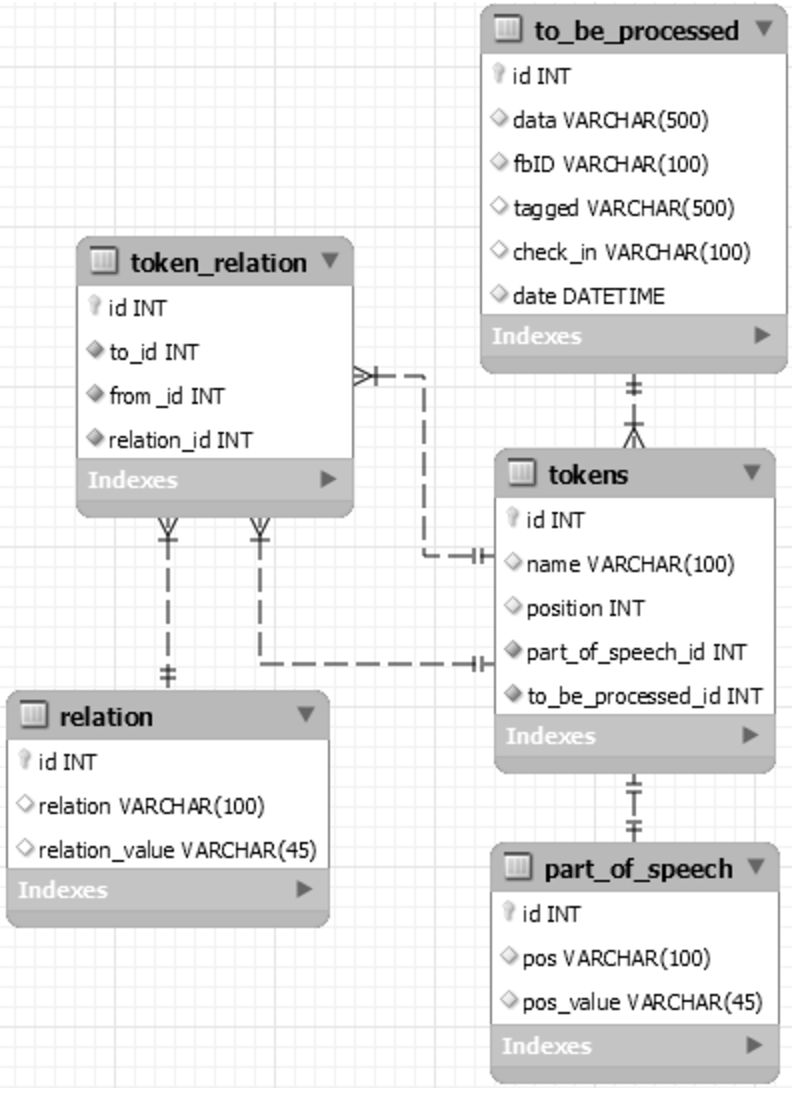
\includegraphics [width=3in,height=3in,keepaspectratio] {dbdesign.png}      %-- include image file named as "disneychart.png" 
	\caption{Database design for storing the processed data.}
	\label{fig:dbdesign}
\end{figure}

\subsection{Knowledge Base}
A knowledge base contains commonsense knowledge needed for content determination in the Text Generation phase. Furthermore, the knowledge base contains the set of templates or ruleset needed when generating the introduction and the conclusion of the life story, as well as the the common sense knowledge that are needed for the body of the life story. The design of the knowledge base is shown in \figref{fig:KnowledgeBaseDB}.

\begin{figure}[!htb]                %-- use [t] to place figure at top, [b] to place at the bottom, [h] for here
   \centering                    %-- use this to center the figure
   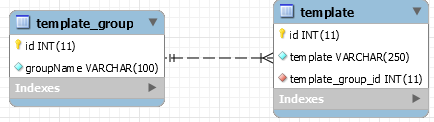
\includegraphics [width=3in,height=3in,keepaspectratio] {TemplateDB.png}      %-- include image file named as "disneychart.png" 
   \caption{Database design for the knowledge base.}
    \label{fig:KnowledgeBaseDB}
\end{figure}

The \textit{Template Group Table} (Table \ref{tab:TemplateGrp}) will contain the different types of templates that can be used for the introduction of a story. It has the following fields:
\begin{itemize}
\item id - unique value that identifies a template group
\item groupName - unique name of the group of templates
\end{itemize}

\begin{table}[ph!]   %t means place on top, replace with b if you want to place at the bottom
\centering
\caption{Sample data in the template\_group table.} \vspace{0.25em}
\begin{tabular}{|p{1cm}|p{6cm}|} \hline
\textbf{id} & \textbf{groupName} \\ \hline
1 & INTRODUCTION \\ \hline
2 & OPTIONAL CLAUSE \\ \hline
3 & BIRTH CIRCUMSTANCES \\ \hline
4 & CONCLUSION \\ \hline
\end{tabular}
\label{tab:TemplateGrp}
\end{table}

The \textit{Template Table} (Table \ref{tab:Template}) will contain all the possible templates for each template group. It has the following attributes.
\begin{itemize}
\item id - unique value that identifies a template
\item groupID - value (corresponding to the id from the template group table) representing the template group in which the template is part of
\item template - the actual template to be used for story text generation
\end{itemize}

\clearpage
\begin{table}[ph!]   %t means place on top, replace with b if you want to place at the bottom
\centering
\caption{Production rile of the introductory and conclusion part of a life story.} \vspace{0.25em}
\begin{tabular}{|p{1cm}|p{2cm}|p{7cm}|} \hline
\textbf{id} & \textbf{groupID} & \textbf{template} \\ \hline
1 & 1 & $<$name$>$ $<$OPTIONAL CLAUSE$>$ $<$BIRTH CIRCUMSTANCES$>$ \\ \hline
2 & 2 & ``a $<$age$>$-year old $<$gender$>$'' \\ \hline
3 & 3 & ``born on'' $<$birth\_date$>$'' \\ \hline
4 & 4 & ``$<$name$>$ likes to listen to music such as $<$page$>$, $<$page$>$, and $<$page$>$.'' \\ \hline
\end{tabular}
\label{tab:Template}
\end{table}

The introductory part of a life story will contain a set of grammar rules in which altogether comprises the introductory template. The introduction part describes the user through the factual information extracted from his/her Facebook profile and stored in the \textit{Direct Knowledge} table. The story would introduce the user's (1) name, birth circumstances as well as the age and nickname/s of the user if provided (2) location and educational background if available and lastly, (3) relationships between other Facebook users. 

The conclusion part will also use a set of grammar rules which would be the basis for constructing the story text that describes the list of preferences of the user. The list of preferences are inferred from the user's likes and stored in the Interest Preferences table. 

The basic structure of a grammar rule that can be used for the introduction and conclusion is found in Table \ref{tab:ProdRule}. The complete list is found in Appendix \ref{sec:appendixj}.

\begin{table}[ph!]   %t means place on top, replace with b if you want to place at the bottom
\centering
\caption{Production Rule of the Introductory Part of a Life Story.} \vspace{0.25em}
\begin{tabular}{|p{1.5in}|p{4in}|} \hline
INTRODUCTION & $<$FIRST$>$ $<$SECOND$>$ $<$THIRD$>$ \\ \hline
FIRST & $<$name$>$ $<$OPTIONAL\_CLAUSE$>$ $<$DESCRIPTION\_OF\_CURRENT\_JOB/EDUCATION$>$ $|$ $<$name$>$ $<$OPTIONAL\_CLAUSE$>$ $<$BIRTH\_C IRCUMSTANCES$>$ \\ \hline
CONCLUSION & ``$<$name$>$ likes to listen to music such as $<$page$>$, $<$page$>$, and $<$page$>$.'' \\ \hline
\end{tabular}
\label{tab:ProdRule}
\end{table}

Template-based text generation will be used to generate the introductory part of a story. Thus, the non-terminal, in the INTRODUCTION production rule, has an associated set of templates that can be used to generate the actual story text. Appendix \ref{sec:appendixk} shows these templates, as well as the the data which will come from the direct knowledge database. A sample resulting sentence is also shown.

\subsection{Text Generation}
The text generation module is responsible for generating the appropriate story segments that make up the entire life story generated by \systemname.

There are three components of the text generation modules, namely the GenIntro, GenBody, and GenConclusion. GenIntro is applied to the data determined to be ``facts'' or direct knowledge. It involves checking the knowledge base for the appropriate template to be used based on the available facts in the direct knowledge table. If there is more than one template available then one template would be randomly chosen from the list of templates. GenIntro would also involve filling the template with the correct data. The generated text will become the introductory paragraph of the life story.

GenBody, on the other hand, is applied to generate the body of the life story from the data processed in the Data Processing module. The body paragraph(s) will be narrating one or more events about a person’s life. These events will be taken from data that users have written and posted on their own Timeline. For these data, text generation is more complex. It will undergo three sub-modules, which are all detailed in Section 3.5.1, Text Generation. Each activity in each sub-module is discussed below.

From the data forwarded by the Pre-Processing module, content determination will now classify all the verbs stored in the \textit{Verb Object} table according to type (e.g. all ``eating” together, then all ``travelling to”, then all ``celebrating”). Because a single post can contain multiple verbs or words signifying events, it can be classified into multiple categories. For example, the post, ``\textit{walking around the streets of Rome while eating delicious gelato.}” is classified as eating and travelling.

From the given sample post above, the verb is identified to be ``write”. To be able to determine the post type, it will check the \textit{Post Type} table for the corresponding id of the verb and update the post\_type column in the \textit{Verb Object} table. After the post classification module, the \textit{Verb Object} table (shown in Table  \ref{tab:sampleUpVO}) now contains the updates data.

\clearpage
\begin{table}[ph!]   
\centering
\caption{Sample data in the updated verb object table.} \vspace{0.25em}
\begin{tabular}{|p{1cm}|p{1in}|p{1.5cm}|p{1in}|p{1in}|} \hline
\textbf{id} & \textbf{post\_id} & \textbf{verb} & \textbf{noun} & \textbf{sentence}\\ \hline
1&1&write&thesis paper document&writing our thesis paper document \\ \hline
\end{tabular}
\label{tab:sampleUpVO}
\end{table}
\begin{table}[ph!]   
\centering
\begin{tabular}{|p{1in}|p{1.2in}|p{1.2in}|p{1in}|} \hline
\textbf{post\_type} & \textbf{tagged}& \textbf{location} & \textbf{date}\\ \hline
15(writing)&Janica Mae Lam, Camille Saavedra, Alds Hade&Gokongwei Building, De La Salle University& 11/22/2016 \\ \hline
\end{tabular}
\end{table}

However, in case of there is no verb present in the post, a reference table (shown in Appendix \ref{sec:appendixl}) containing predefined keywords commonly associated with each event category that was derived through manual inspection of the dataset will be used to classify the post type. For \textit{celebrating} events, words which usually indicate special events such as birthdays and Christmas are used. For posts on \textit{travelling}, synonyms as well as methods of traveling are used. For \textit{eating}, aside from synonyms, the meals of the day are also used as indicators.

All post types stored in the \textit{Verb Object} table will first be sequenced according to date (newest post first) but may be presented in a different paragraph (depending on the post type). Additionally, if there is an event stored in the Verb Object table with the same date as the predefined activity, then the content determination may infer that both activities occurred on the same period of time and arrange this in the story in the order they were posted.

For every classified post in the \textit{Verb Object} table (Table \ref{tab:sampleVO}), content determination will now construct a message for each of it. For each constructed message, it would be comprised of the object from the \textit{Verb Object} table pertaining to the said verb together with the tagged, date and location of with whom, when and where the event has happened which is also stored in the to \textit{Verb Object} table.

With the sample event in \textit{Verb Object} table (Table \ref{tab:sampleUpVO}), content determination can generate the message write(Robee Khyra Te, thesis paper document, Janica Mae Lam, Camille Saavedra, Alds Hade, 11/22/2016, Gokongwei Building, De La Salle University - Manila). 

The final output of the content determination will be an abstract representation of the story plan that is composed of a set of messages or predicates that the system would like to convey to the reader. Each message in the story plan will follow the abstract representation of the form:
\begin{center}Verb(doer, receiver, object, date, location) \end{center}

Given the story plan from content determination, sentence aggregation will then determine how the messages in the story plan can be combined to form a single sentence, as well as the relationship across two sentences based on rhetorical structure theory (Section 3.5.2.2 - Rhetorical Relations). Appropriate discourse markers will then be used, such as and, therefore, but, because, to name a few, in order to show if one sentence is used to explain, justify, elaborate or provide an example to another sentence. Pronoun generation will also be done in this process. 

Sentence Aggregation will also be responsible for determining the time elements of a message. Specifically, these time elements include ``last $<$year/month/week$>$'' ``every $<$year/month/week$>$'', ``often'', ``recently'', ``$<$n$>$ week(s)/month(s)/year(s) ago'', and ``every $<$n$>$ day(s)/week(s)/month(s)/year(s)''. For example, all messages reflecting events that happened in the past month will be aggregated together by the time element ``last month''.

Lastly, linguistic realization will be responsible for generating the surface form of the story text using SimpleNLG. SimpleNLG would also be used to automate the following realization tasks:
\begin{enumerate} [label=\alph*.]
\item Orthography - This would include inserting appropriate spaces in sentences or paragraphs, correct usage of punctuation marks, among others.
\item Morphology - This includes modifying or changing the word to reflect grammatical information such as gender, tense, number or person.
\item Simple Grammar - This includes ensuring grammatical correctness by checking the subject-verb agreement, creating a well-formed verb groups and connecting different parts of a sentence together into an appropriate syntactic structure.
\end{enumerate}

GenConclusion will be used to generate the conclusion part of the story text, which will contain the user's likes and preferences. The exact process of determining the user's likes is explained in the Inferencing Section, 4.4.4. Similar to the approach in GenIntro, GenConclusion would check the available templates defined in the Template table and use the data stored in the interest preferences table.

\subsection{Generate Output}
The generated texts from the two text generation modules are then merged, and presented to the user as the complete life story. The user will now have the option to save or discard his/her life story. If the user wishes to save his/her life stories, a text file will be created and the user chooses where to save this file. But if the user wishes to discard this, then he/she simply closes the software.

%section~~~~~~~~~~~~~~~~~~~~~~~~~~~~~~~~~~~~~~~~~~~~~~~~~~~~~~~~~~~~~~
\section{Software Functions}
\systemname provides a simple environment that allows users to easily use it to create a life story from their Facebook posts and save these stories for future use. Below are the software functions used in \systemname.

\subsection{Login Window}
In using the application, the user would have to Login to Facebook for the software to access the data stored in his/her account. A Facebook login button would prompt the user to login as shown in \figref{fig:Login}. Once the button is clicked, a Login Window, which can be seen in \figref{fig:Login2}, would pop up informing the user that he/she is logging in his/her Facebook account with the app, StoryBook. Login information such as email address, phone number or user id along with the corresponding password are both needed to successfully login. 

Logging in to the app also grants the permissions set by the app which then automatically updates the access token stored in cookies. 

\begin{figure}[!htb]                %-- use [t] to place figure at top, [b] to place at the bottom, [h] for here
   \centering                    %-- use this to center the figure
   
\includegraphics [width=3in,height=2in,keepaspectratio] {login1.png}      %-- include image file named as "disneychart.png" 
   \caption{Facebook Login Button.}
    \label{fig:Login}
\end{figure}

\begin{figure}[!htb]                %-- use [t] to place figure at top, [b] to place at the bottom, [h] for here
   \centering                    %-- use this to center the figure
   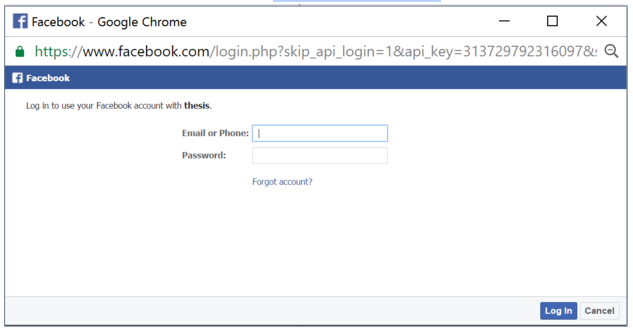
\includegraphics [width=\textwidth] {login2.png}      %-- include image file named as "disneychart.png" 
   \caption{Pop-up Login Window.}
    \label{fig:Login2}
\end{figure}

Logging in to the app also grants the permissions set by the app which then automatically updates the access token stored in cookies. 

\subsection{Permission Window}
Logging in to Facebook automatically stores a default access token in cookies. If the user is already logged-in on Facebook and the \systemname automatically obtains the user's access token, then it would check permissions in the access token and prompts the user of the missing permissions it needs to acquire. \figref{fig:Permission} displays the permission window that asks the user to grant the permissions needed by the software.

\begin{figure}[!htb]                %-- use [t] to place figure at top, [b] to place at the bottom, [h] for here
   \centering                    %-- use this to center the figure
   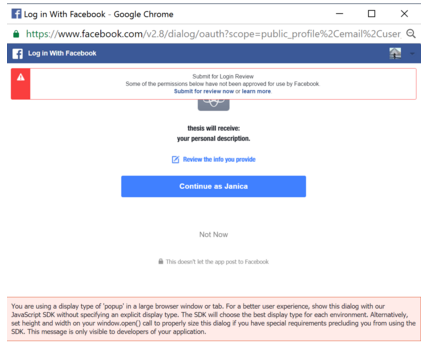
\includegraphics [width=\textwidth] {permission.png}      %-- include image file named as "disneychart.png" 
   \caption{Permission Window.}
    \label{fig:Permission}
\end{figure}

\subsection{Generated Story Output Window}
The Generated Story Output Window, \figref{fig:Output}, is basically a window that displays the generated story after \systemname has analyzed and processed the gathered data from the user's Facebook account. The user would be given an option to save the generated story to a text file through the ``Save to Text File" button.

\begin{figure}[!htb]                %-- use [t] to place figure at top, [b] to place at the bottom, [h] for here
   \centering                    %-- use this to center the figure
   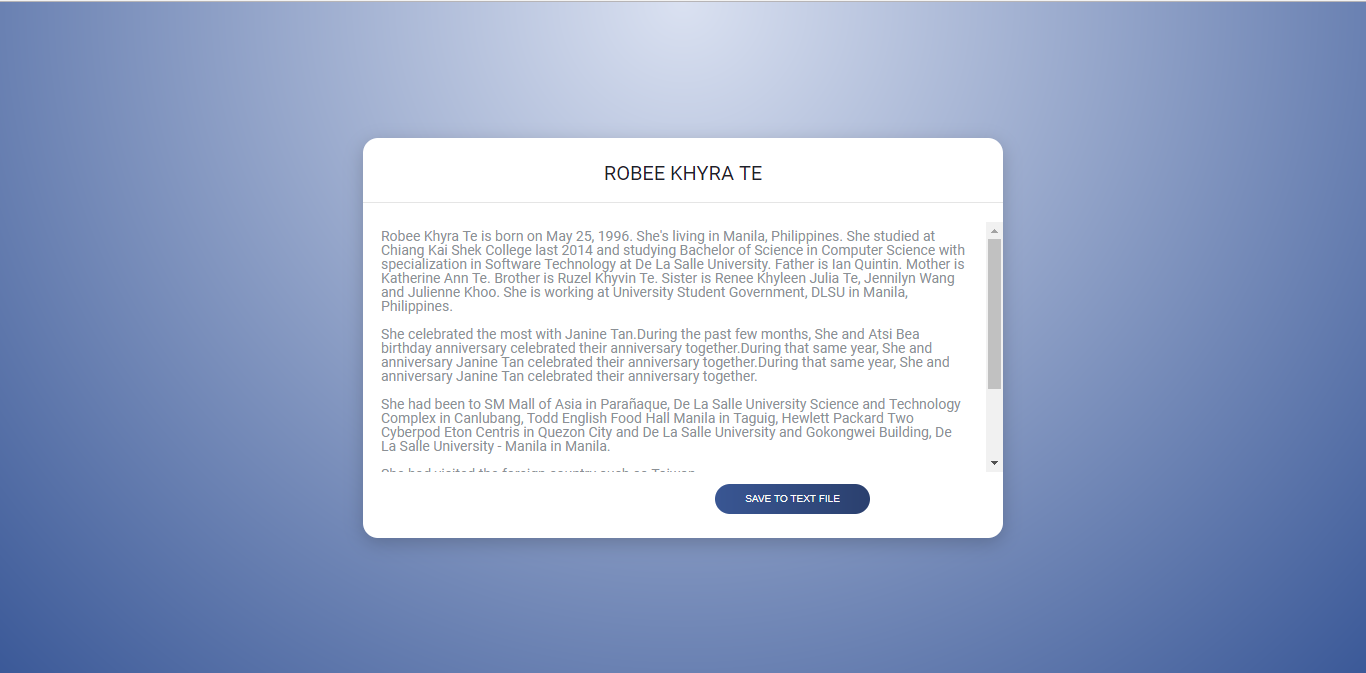
\includegraphics [width=\textwidth] {GeneratedStoryOutputWindow.png}      %-- include image file named as "disneychart.png" 
   \caption{Generated Story Output Window.}
    \label{fig:Output}
\end{figure}

\section{Physical Enviroment and Resources}
This section details the minimum and recommended software requirements for software implementation.

\systemname requires the following resources for development:
\begin{itemize}
\item Eclipse IDE
\item MySQL Server and Workbench
\item Java Development Kit (JDK)
\item Apache Tomcat 8.0
\end{itemize}

These are the minimum software requirements for \systemname to run properly:
\begin{itemize}
\item \textbf{OS}: Windows 8.1 / 10
\item \textbf{Memory}: 1 GB RAM
\item \textbf{Storage}: At most 1 GB of free hard disk space
\item \textbf{Internet connection}: Broadband, at least 1Mb/s bandwidth
\item \textbf{Others}: Java Runtime Environment (JRE), MySQL Server, Apache Tomcat 8.0
\end{itemize}

\subsection{Tools}
The following tools will be used for the development and runtime of the \systemname.

\subsubsection{Facebook Login API}
The Facebook Login API enables the use of the Facebook user's identity in order to craft interesting stories about them. It enables the application to extract data from Facebook to be processed and used to generate stories. Features of Facebook Login, such as access tokens and permissions, make it safe and secure for people and apps to use, but there are some security steps which this software will need to implement. This will be tackled in Chapter 5, Design and Implementation.

\subsubsection{Graph API}
The use of Graph API enables the software to extract posts and data from a specific Facebook account. It supports developers by supplying services such as providing snippets of codes for easier integration with JSON requests and responses.

\subsubsection{Stanford CoreNLP}
Stanford CoreNLP will be used in the text understanding module, as it provides the needed component, syntax analysis. 

\subsubsection{WordNet}
WordNet will be used to supply the data that is needed for the reference table which contains keywords such as related verbs and nouns. The reference table will then be used in the classification of Facebook post which does not contain a verb.

\subsubsection{ConceptNet}
ConceptNet is a semantic network containing concepts with Open Mind Common Sense as its main source of knowledge, along with other sources such as Wikipedia, WordNet, and DBPedia. This knowledge will be used to supply keywords for the reference table to be used in the post classification module. This will gather related verbs and noun for the categories \textit{Celebrating}, \textit{Travelling}, \textit{Eating}, and \textit{Drinking}.

\subsubsection{SimpleNLG}
SimpleNLG will be used in generating grammatically correct English sentences. SimpleNLG will also automate some of the tasks an NLG system needs to perform like checking the orthography, morphology and simple grammar of the sentences.